% ---------------------------------------------------------------------------
% Appendix A: Extended results (supplementary figures).
% Order of the appendix: A extended results -> B detailed methods
% (extended_methods.tex) -> theory (theory_appendix_polished.tex).
% Plan and figure sources: notes/appendix_outline_plan.md.
% Figures not yet exported to figures/ are shown as \suppfigplaceholder boxes
% naming their source in the code repository (AccentuationPredRMT).
% ---------------------------------------------------------------------------

\providecommand{\suppfigplaceholder}[2][0.22\textheight]{%
  \fbox{\parbox[c][#1][c]{0.95\linewidth}{\centering\small
  \textcolor{magenta}{\textbf{[figure to insert]}}\\[2pt]
  \texttt{\detokenize{#2}}}}}

\section{Extended results}
\label{sec:app-extended-results}

The appendix has three parts.  This section collects supplementary figures
that extend the main-text figures.  Section~\ref{sec:app-methods} describes
the numerical experiments and the neuronal analyses in detail.  The theory
follows from Section~\ref{sec:app-theory-roadmap} on: every result stated in
derivation order, then proofs grouped by topic.

% ---------------------------------------------------------------------------
\subsection{Geometry of the ridge path}
\label{sec:app-ext-geometry}
% Supports Fig.~\ref{fig:geometry} (Sec.~\ref{sec:setup}) and the ridge-path
% paragraph of Sec.~\ref{sec:pixel}.  Theory: Prop.~\ref{prop:mr-iso-geometry},
% Exp.~\ref{ex:mr-dissociation}.  Methods: App.~\ref{sec:app-methods-geometry}.
\todo{One paragraph: exact conditional Gaussian of $\bhat\mid X$ in the plane of
a high- and a low-variance PC; (a) varying $\sigma^2$ at fixed $\lambda$,
(b) varying $\lambda$ at fixed $\sigma^2$; prediction-stationary point vs.\
$z=0$ crossing.}

\begin{figure}[ht]
\centering
\suppfigplaceholder{figures/geometry/ridge_paths_iso_error_geometry.pdf  (fix literal "68\%" in legend, overlapping teacher label)}
\caption{\textbf{Exact conditional geometry of ridge estimators in two
dimensions.} \todo{caption} Setting in App.~\ref{sec:app-methods-geometry}.}
\label{fig:supp-ridge-path-geometry}
\end{figure}

% ---------------------------------------------------------------------------
\subsection{Pixel-space ridge on natural images}
\label{sec:app-ext-pixel}
% Supports Fig.~\ref{fig:pixel} (Sec.~\ref{sec:pixel}).
% Methods: App.~\ref{sec:app-vanhateren-landscape-methods}.
% Theory: App.~\ref{sec:app-pixel-ridge}, \ref{sec:app-optimal-regularization},
% \ref{sec:app-ratio-corrections}.
\todo{Short text: (i) DE vs.\ natural-image Monte Carlo over the full
noise--regularization plane; (ii) slope landscapes; (iii) fixed penalty
vs.\ CV-selected vs.\ control-oracle penalty along the noise axis, including
where the leading DE fails (near the control optimum) and the Gaussian
surrogate of App.~\ref{sec:app-ratio-gaussian} takes over.}

\begin{figure}[ht]
\centering
\suppfigplaceholder{figures/vanhateren_landscape/export/composite/paper_composite_three_landscapes_de_mc_rows_figexport.pdf  (crop to the 2x3 heatmaps)}
\caption{\textbf{Deterministic equivalents versus natural-image Monte Carlo
for the landscapes of Fig.~\ref{fig:pixel}.} \todo{caption}}
\label{fig:supp-pixel-de-mc}
\end{figure}

\begin{figure}[ht]
\centering
\suppfigplaceholder{figures/vanhateren_landscape/landscape_slope_kappa.pdf}
\caption{\textbf{Slope landscapes} of generalization and accentuation, DE
(top) and Monte Carlo (bottom). \todo{caption}}
\label{fig:supp-pixel-slope}
\end{figure}

\begin{figure}[ht]
\centering
\suppfigplaceholder[0.3\textheight]{notebooks/outputs/pixel_ridge/vanhateren_selection_estimation/selection_vs_estimation_extended_with_sklearn_cv.pdf}
\caption{\textbf{Fixed, prediction-selected and control-selected penalties
along the noise axis.} \todo{caption; leading DE vs.\ Gaussian surrogate vs.\
MC; empirical LOOCV}}
\label{fig:supp-pixel-selection}
\end{figure}

% Q6 (decide later): synthetic isotropic / power-law validation of the
% generalization, accentuation and peer DEs (figures/peer_validation/
% r2_peer_validation.png; figures/model_selection/cv_selected_r2.png).
% \label{fig:supp-synthetic-validation}

% ---------------------------------------------------------------------------
\subsection{Linear feature ridge: the prediction-null family}
\label{sec:app-ext-gauge}
% Supports Fig.~\ref{fig:feature} (Sec.~\ref{sec:feature}).
% Theory: App.~\ref{sec:app-gauge-fragility} (Prop.~\ref{prop:app-feature-gauge},
% Cor.~\ref{cor:mr-rotation}); full dependency graph stays in theory as
% Fig.~\ref{fig:summary_stats_dep_graph}.  Methods: App.~\ref{sec:app-methods-feature}.
\todo{Short text: continuous rotation from top-$p$ PC projectors
(Fig.~\ref{fig:app-null-rotation}); random draws from the family
(Fig.~\ref{fig:supp-null-random}); what the rotation does to individual
feature rows (Fig.~\ref{fig:supp-null-row-spectra}); dependence on the
feature dimension $p$ (Fig.~\ref{fig:supp-null-dimension}).}

\begin{figure}[ht]
\centering
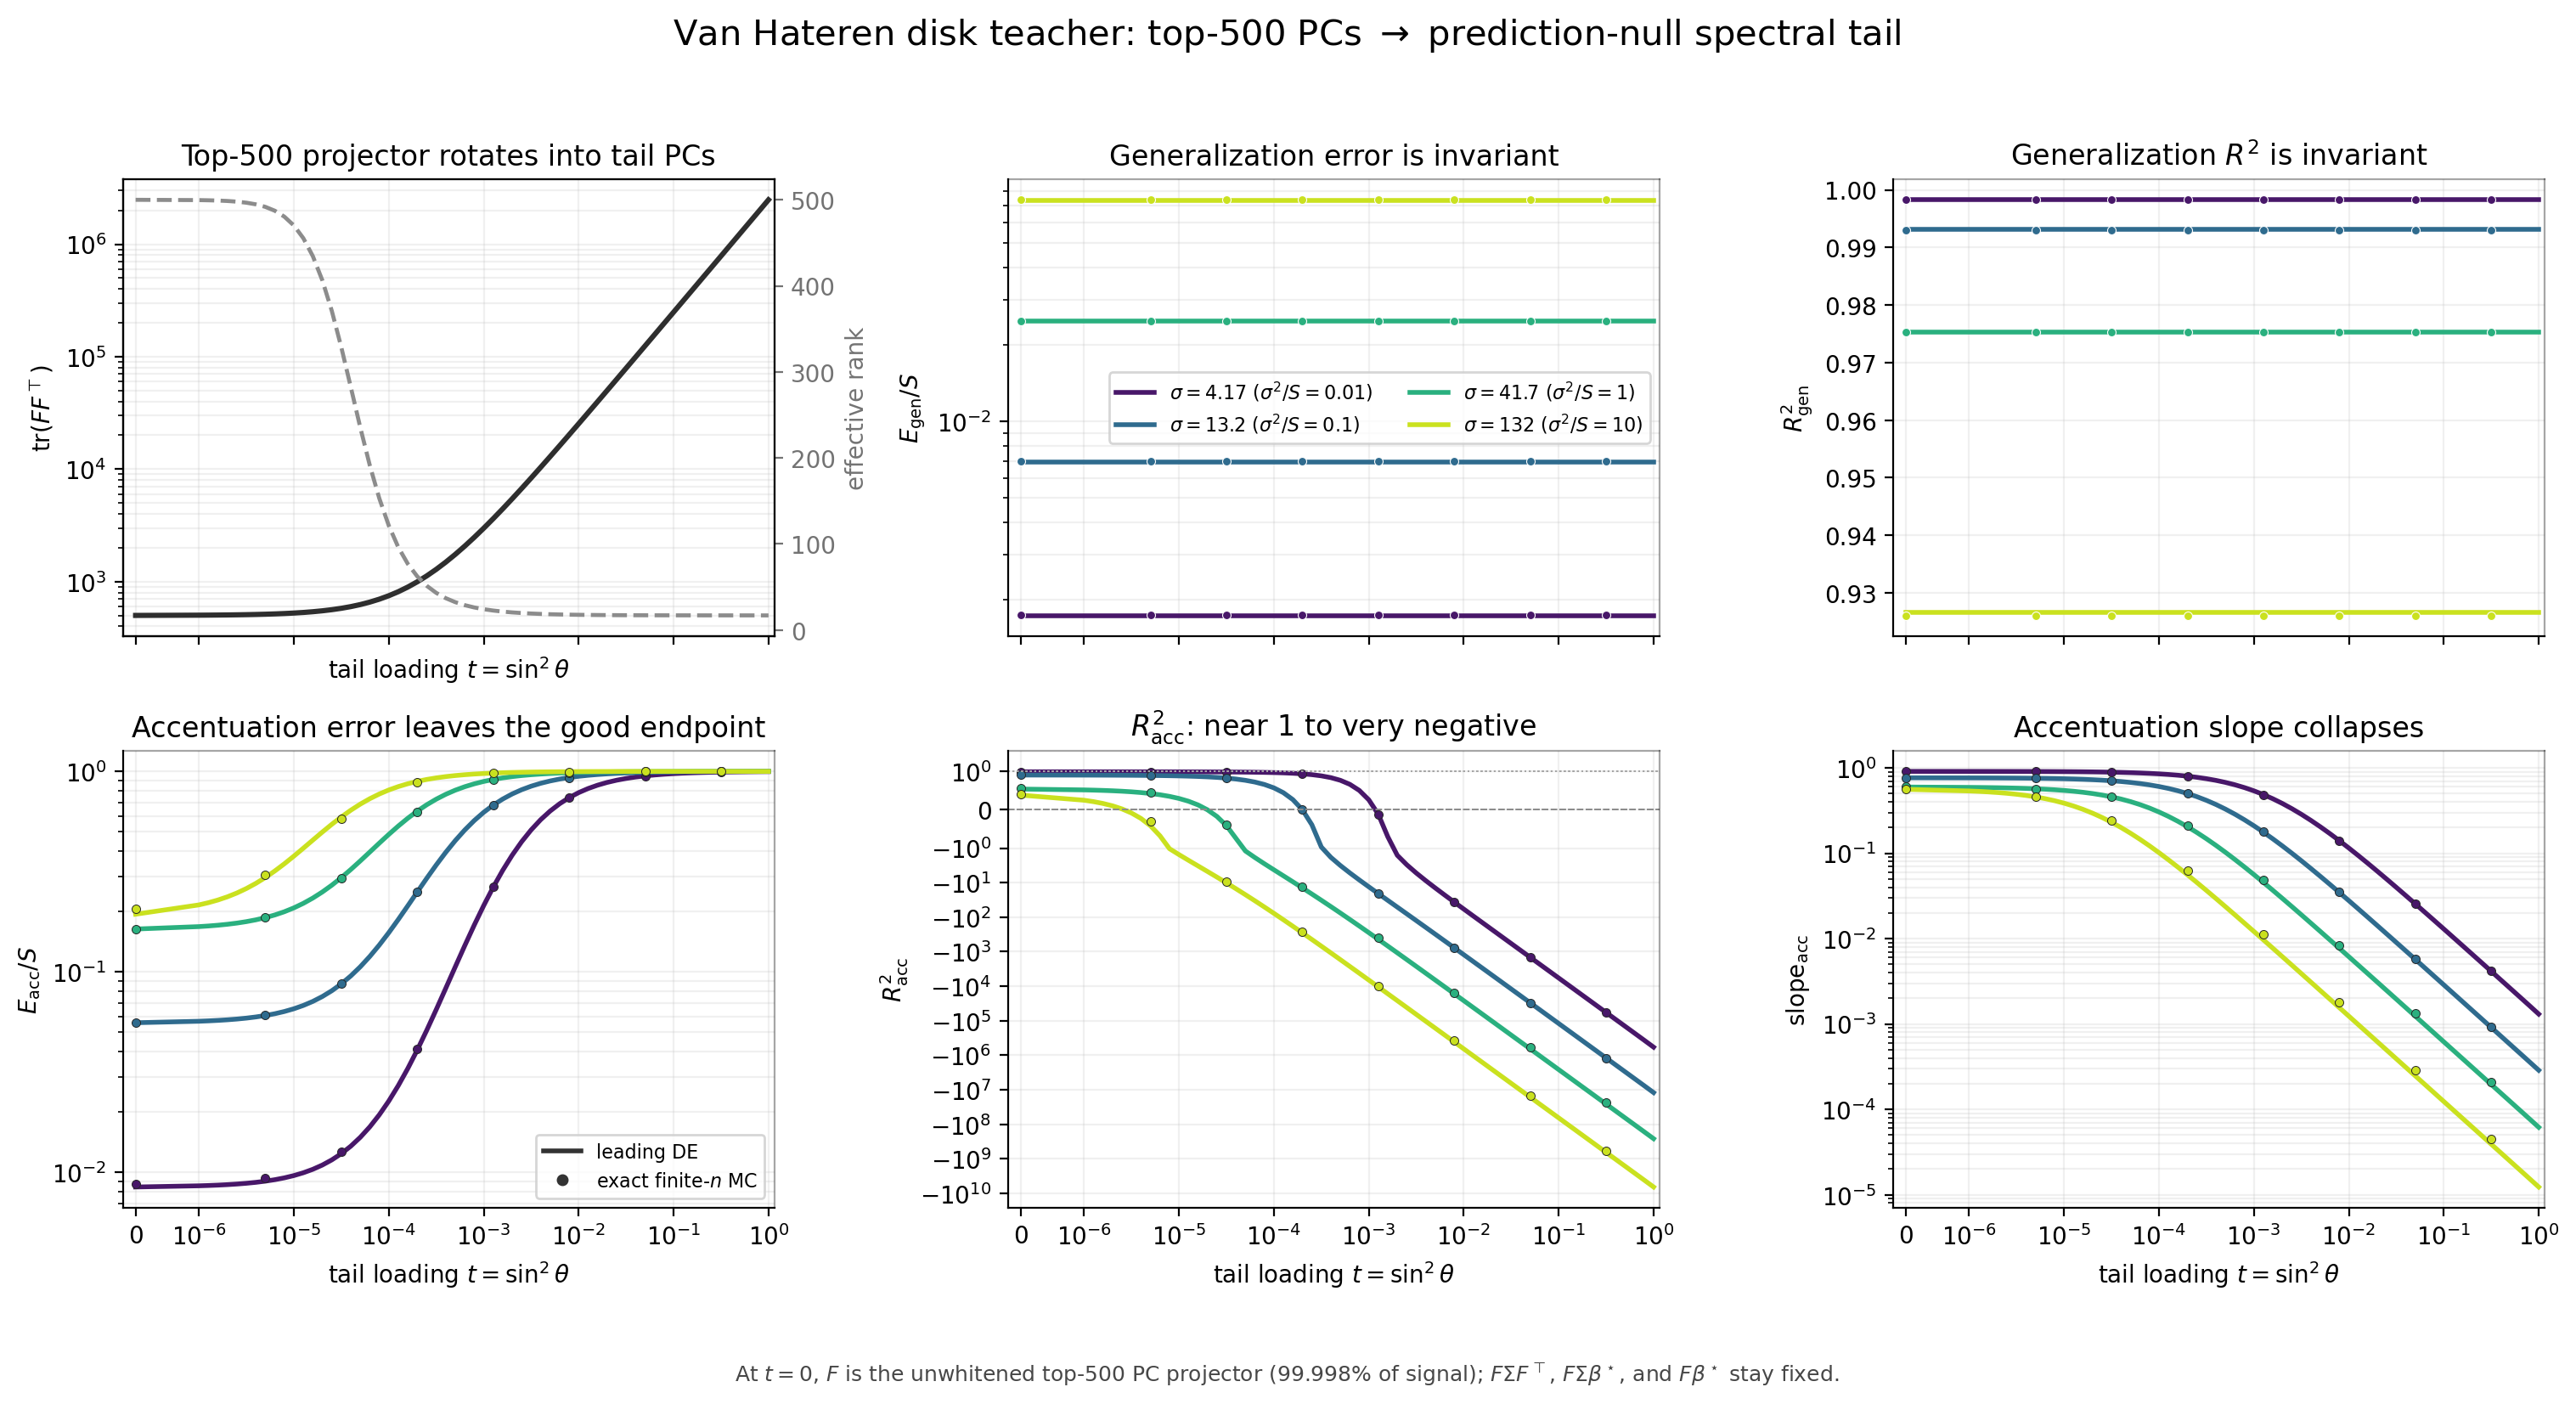
\includegraphics[width=1\linewidth]{figures/VanHateren_Top500PC_prediction_null_feature_rotation}\\
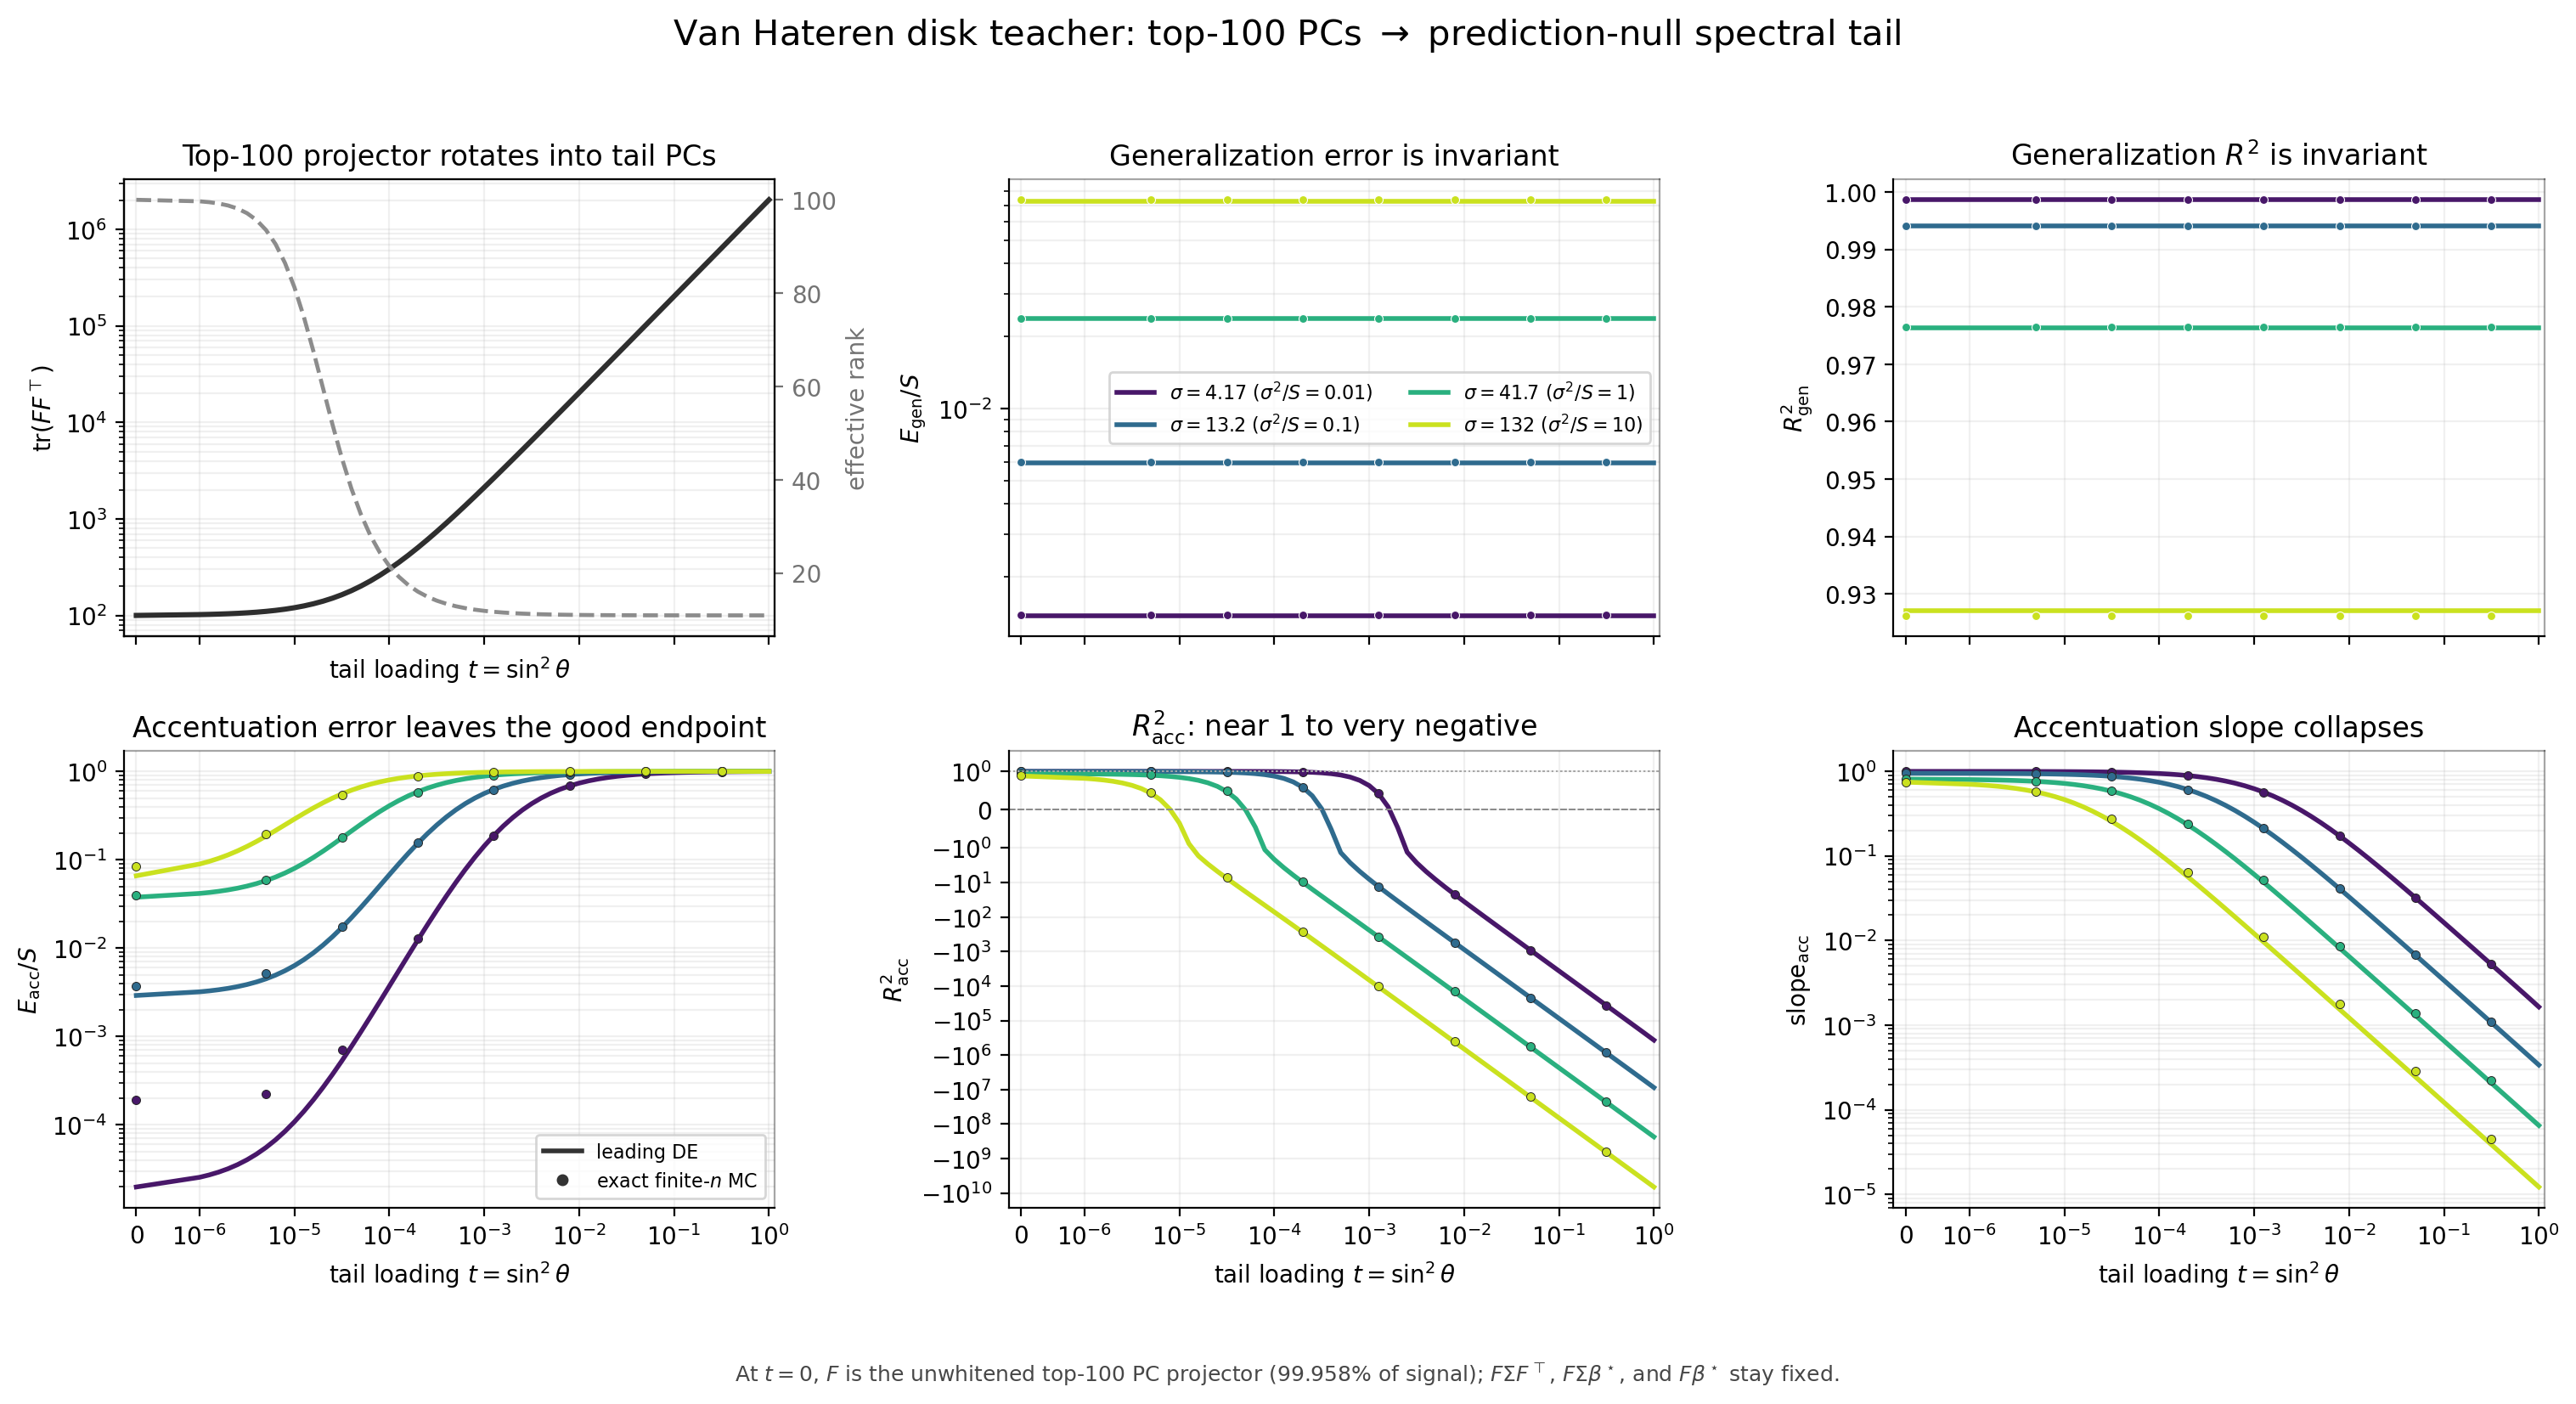
\includegraphics[width=1\linewidth]{figures/VanHateren_Top100PC_prediction_null_feature_rotation}
\caption{\textbf{Continuous prediction-null rotation on van Hateren images}
(Corollary~\ref{cor:mr-rotation}), starting from the top-500 (top) and
top-100 (bottom) PC projectors and rotating their null part into the
spectral tail.  Generalization error, $R^2_{gen}$ and the selected penalty are
exactly constant in the tail loading $t$, while $\operatorname{Tr}(FF^\top)$,
accentuation error, $R^2_{acc}$ and slope change by orders of magnitude.
Lines: leading DE; markers: finite-$n$ Monte Carlo.}
\label{fig:app-null-rotation}
\end{figure}

\begin{figure}[ht]
\centering
\suppfigplaceholder{figures/null_rotations/vanhateren_p500_random_null_diversity.pdf}
\caption{\textbf{Random maps from the prediction-null family ($p=500$).}
\todo{caption: identical $E_{gen}$, $R^2_{gen}$; accentuation metrics
spread over orders of magnitude with $\operatorname{Tr}(FF^\top)$.}}
\label{fig:supp-null-random}
\end{figure}

\begin{figure}[ht]
\centering
\suppfigplaceholder{figures/null_rotations/vanhateren_top_pc_tail_feature_spectra.pdf}
\caption{\textbf{Spectral location of individual feature rows along the
rotation.} \todo{caption}}
\label{fig:supp-null-row-spectra}
\end{figure}

\begin{figure}[ht]
\centering
\suppfigplaceholder{figures/null_rotations/vanhateren_null_dimension_curves.pdf}
\caption{\textbf{Null rotation across feature dimension $p$.} \todo{caption:
leading DE vs.\ Gaussian distributional DE vs.\ MC.}}
\label{fig:supp-null-dimension}
\end{figure}

% ---------------------------------------------------------------------------
\subsection{Peer review in the neuronal experiment}
\label{sec:app-ext-peer}
% Supports Sec.~\ref{sec:phenomena} (recognition without generation) and the
% peer-review paragraph of Sec.~\ref{sec:pixel}.  Theory:
% App.~\ref{sec:app-peer-review}, \ref{sec:app-peer-shared}.
% Methods: App.~\ref{sec:app-methods-peer}.
\todo{Short text: generator $\times$ reviewer matrices; self (diagonal) vs.\
peer (off-diagonal) distributions and tests.}

\begin{figure}[ht]
\centering
\suppfigplaceholder{figures/nonlinear_control/neural_peer_review/peer_review_four_metrics_jacob_order.pdf}
\caption{\textbf{Neuronal peer review.} Rows: generating model; columns:
reviewing model; diagonal: self-evaluation. \todo{caption}}
\label{fig:supp-neural-peer-matrix}
\end{figure}

\begin{figure}[ht]
\centering
\suppfigplaceholder{NEW: self vs peer R^2 and slope distributions (stats in tables/nonlinear_control/.../PEER_REVIEW_SELF_VS_PEER_RESULTS.md)}
\caption{\textbf{Self-evaluation versus peer review.} \todo{caption}}
\label{fig:supp-neural-self-vs-peer}
\end{figure}

% ---------------------------------------------------------------------------
\subsection{Nonlinear gradient diagnostic: full comparison}
\label{sec:app-ext-nonlinear}
% Supports Fig.~\ref{fig:nonlinear-biological-validation} (Sec.~\ref{sec:nonlinear}).
% Theory: App.~\ref{sec:app-nonlinear-diagnostic}.
% Methods: App.~\ref{sec:app-methods-models}, \ref{sec:app-methods-nonlinear},
% \ref{sec:app-methods-stats}.
\todo{Short text: per-model gradient geometry; all estimators and
neighborhood scales; dependence on smoothing scale; robustness to
residualization, predictor transform and session endpoint.}

\begin{figure}[ht]
\centering
\suppfigplaceholder[0.3\textheight]{NEW: per-model s_k, q_k=||J^T v_k||^2, q_k/s_k, cumulative T at df_2=375, one panel per model (data: mass_v1/geometry/*/summary.npz)}
\caption{\textbf{Gradient geometry of the ten encoding models.}
\todo{caption}}
\label{fig:supp-model-spectra}
\end{figure}

\begin{figure}[ht]
\centering
\suppfigplaceholder[0.3\textheight]{figures/nonlinear_control/biological_validation/site_centered_predictor_benchmark_control_session_pearson_fdr.png}
\caption{\textbf{All candidate predictors of control.} \todo{caption:
estimators $\times$ scales $\times$ model subsets, slope and control MSE.}}
\label{fig:supp-nonlinear-benchmark}
\end{figure}

\begin{figure}[ht]
\centering
\suppfigplaceholder{figures/nonlinear_control/biological_validation/site_centered_{smooth,neighborhood}_correlations.png  and/or forward_noise/noise_geometry.pdf}
\caption{\textbf{Dependence on the neighborhood scale $\tau$.} \todo{caption}}
\label{fig:supp-smoothing-scale}
\end{figure}

\begin{figure}[ht]
\centering
\suppfigplaceholder{pick 2-3: residualization variants; paper_v4_raw_x / paper_v5_raw_predictors; session_endpoint_image_bootstrap.png; ..._encoding_session.png}
\caption{\textbf{Robustness of the within-site association.} \todo{caption}}
\label{fig:supp-nonlinear-robustness}
\end{figure}
